% ICASSP 2027 manuscript. The official spconf style controls the required
% paper size, margins, two-column layout, Times text font, and empty page style.
% Replace the placeholder author and affiliation fields before submission.
\documentclass{article}
\usepackage{spconf,amsmath,amssymb,graphicx,booktabs,multirow}
\usepackage{placeins,float}
\usepackage[nospace]{cite}
\renewcommand{\citedash}{]\textendash[}
\renewcommand{\citepunct}{],\penalty\citepunctpenalty\ [}
% Keep links active in the PDF without introducing colored boxes in the
% camera-ready print layout.
\usepackage{url}
\usepackage[hidelinks]{hyperref}
% Relax float constraints so the two large top floats (Fig. 3 and Table 2)
% can share the top of the last content page.
\renewcommand{\topfraction}{0.95}
\setcounter{topnumber}{3}
\setcounter{totalnumber}{5}
\renewcommand{\textfraction}{0.05}
\renewcommand{\floatpagefraction}{0.85}
\renewcommand{\dbltopfraction}{0.95}
\setcounter{dbltopnumber}{3}
\renewcommand{\dblfloatpagefraction}{0.85}
\newcommand{\metrictriplet}[3]{\makebox[3.1em][c]{#1}\hspace{0.5em}\makebox[3.1em][c]{#2}\hspace{0.5em}\makebox[3.1em][c]{#3}}
\newcommand{\metricheader}{\makebox[3.1em][c]{AP}\hspace{0.5em}\makebox[3.1em][c]{AP$_{50}$}\hspace{0.5em}\makebox[3.1em][c]{AP$_{75}$}}

\title{PROMPTMINER-SAM2: PROMPT MINING AND UNCERTAINTY-GUIDED REFINEMENT FOR REMOTE SENSING INSTANCE SEGMENTATION}
\name{Cheng Wang$^{1,2}$, Baotian Shi$^{2}$, Xiaoyu Li$^{1}$, Han Zhang$^{2}$\sthanks{Corresponding author: Han Zhang (zhanghan9937@nwpu.edu.cn).}}
\address{$^{1}$School of Cybersecurity, National School of Secrecy, Northwestern Polytechnical University, Xi'an, China\\
$^{2}$School of Artificial Intelligence, Optics and Electronics (iOPEN), Northwestern Polytechnical University\\Xi'an, China}

\begin{document}
\maketitle

\begin{abstract}
Accurate remote-sensing instance segmentation remains challenging in complex scenes.
Existing methods decode masks from latent candidate representations, without explicitly using shape cues for irregular or adjacent boundaries.
To address this limitation, we propose PromptMiner-SAM2, an end-to-end framework for remote-sensing instance segmentation.
It predicts per-candidate coarse shapes first and mines the resulting shape cues for mask decoding.
Specifically, the coarse shape prompt mining module (CSPM) predicts the coarse shapes from candidate region-level features and generates shape-aware prompts accordingly.
Moreover, a decoder-tail module (UDR) is designed to identify uncertain pixels and correct the predictions using local mask features and instance context.
Experiments on the WHU and NWPU VHR-10 benchmarks show that PromptMiner-SAM2 achieves
mask AP values of 73.4\% and 68.3\%, respectively, attaining the highest mask AP among the compared methods.
\end{abstract}
\begin{keywords}
Instance segmentation, remote sensing, SAM2, prompt mining, mask refinement
\end{keywords}

\section{INTRODUCTION}

Remote-sensing instance segmentation assigns each object a pixel-level mask, supporting urban planning and disaster assessment~\cite{rsiisn,p2pformer}.
High-resolution remote-sensing images exhibit scale variation and complex backgrounds that complicate instance-mask prediction.

Existing methods use two-stage, one-stage, conditional-mask, or set-prediction paradigms and decode masks from region features, dynamic parameters, or instance queries~\cite{maskrcnn,msrcnn,htc,condinst,mask2former}.
In remote sensing, prior work improves masks through multi-scale feature fusion, boundary modeling, and foundation-model adaptation~\cite{rsiisn,p2pformer,rs4d,directsamrs,sopseg}. 
SAM~\cite{sam} and SAM2~\cite{sam2} enable prompt-conditioned mask decoding, while related work explores learned and adapted prompts~\cite{rsprompter,pasam,airwaysam,rs2sam2}.

However, many approaches lack explicit candidate-local shape cues, leaving limited decoder guidance for irregular contours or adjacent instances.
Recent SAM-based methods adapt spatial prompts for remote-sensing instance segmentation~\cite{rsprompter,aopsam,causalsam}, while others refine coarse masks through prompt generation~\cite{samrefiner,samref,promptmoe}.
These studies collectively suggest that explicit shape cues effectively complement instance-mask decoding.
For this purpose, explicit shape cues are introduced into end-to-end remote-sensing instance segmentation, as illustrated in Fig.~\ref{fig:motivation}.


Our main contributions are summarized as follows:

\begin{figure}[t]
\centering
\makeatletter
\long\def\@makecaption#1#2{%
  \vskip 2pt
  \setbox\@tempboxa\hbox{#1. #2}%
  \ifdim \wd\@tempboxa >\hsize #1. #2\par \else \hbox
  to\hsize{\hfil\box\@tempboxa\hfil}%
  \fi}
\makeatother
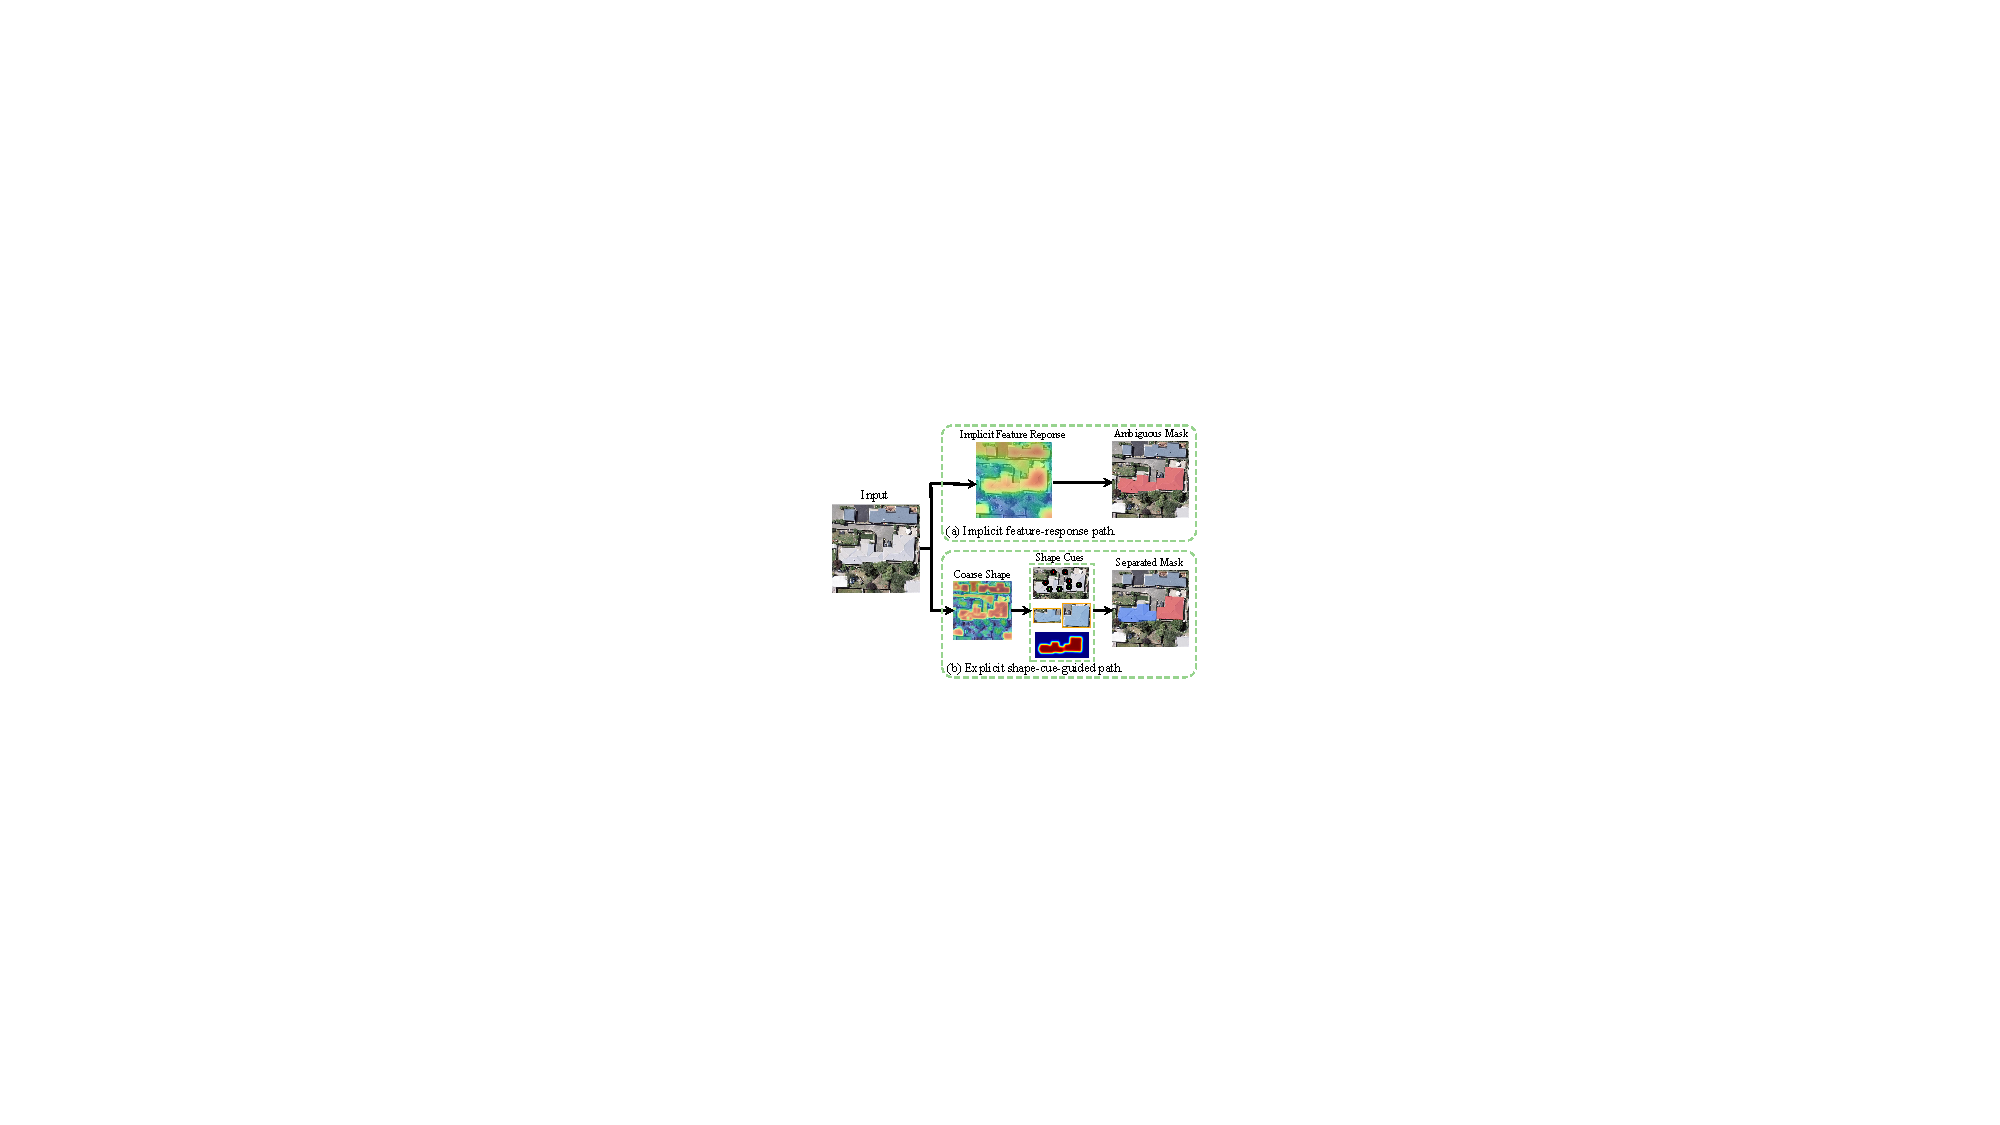
\includegraphics[width=\columnwidth]{A-4.pdf}
\caption{The effect of coarse-shape prompt mining. The path (b) is our approach.}
\label{fig:motivation}
\end{figure}

\begin{figure*}[!t]
\centering
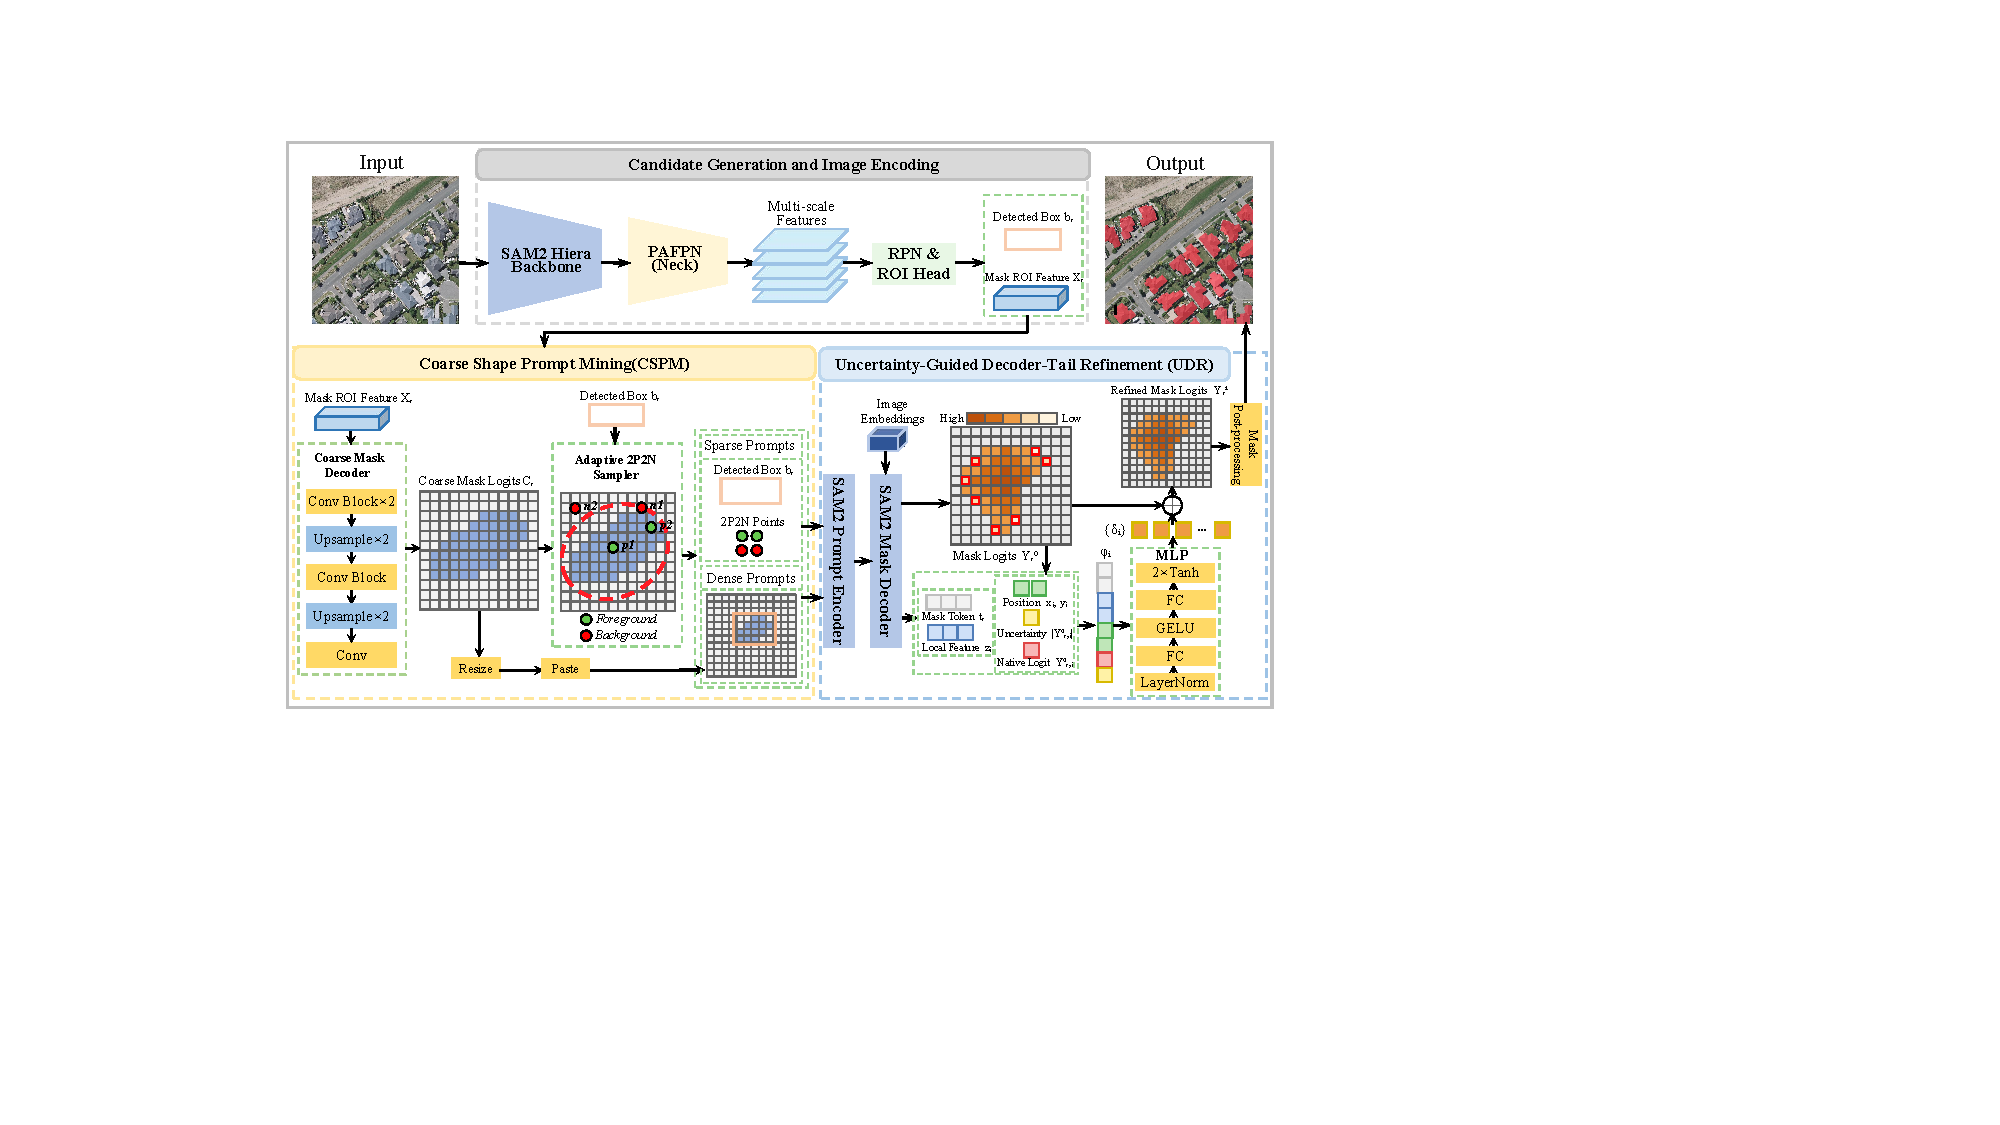
\includegraphics[width=\textwidth]{总体架构图.pdf}
\caption{Overview of the proposed PromptMiner-SAM2. The feature-extraction branch produces candidates, CSPM provides SAM2 with coarse-shape-derived prompts, and UDR corrects uncertain mask pixels.}
\label{fig:arch}
\vspace{-0.8\baselineskip}
\end{figure*}

\begingroup
\vspace{-1.0\baselineskip}
\begin{itemize}\setlength{\topsep}{0pt}\setlength{\partopsep}{0pt}\setlength{\itemsep}{0pt}\setlength{\parsep}{0pt}
  \item We propose \textbf{PromptMiner-SAM2}, a two-stage framework that mines shape cues from per-candidate coarse shapes to form explicit SAM2 prompts for end-to-end remote-sensing mask prediction.
  \item We introduce \textbf{CSPM} and \textbf{UDR}: CSPM predicts a per-candidate coarse shape and mines diverse prompts from it, while UDR selectively corrects low-confidence predictions to improve mask quality.
  \item We conduct extensive experiments on the WHU and NWPU VHR-10 benchmarks, showing the effectiveness of explicit shape cues for mask prediction and uncertainty-driven refinement.
\end{itemize}
\endgroup 

\section{METHOD}
\subsection{Overall Architecture}
Fig.~\ref{fig:arch} illustrates the overall architecture of the proposed PromptMiner-SAM2 for remote-sensing instance segmentation, which couples a two-stage detector with the SAM2 prompt-based mask decoder and associates instance localization to mask prediction in one process.
Given an image $I$, the Hiera encoder of SAM2 extracts multi-scale features. The detection branch produces candidate regions and RoI features through the PAFPN, RPN, and RoI pathways. The same Hiera features serve as image embeddings for subsequent SAM2 mask decoding.
For each candidate, the proposed CSPM predicts a per-candidate coarse shape and mines sparse and dense prompts from it. SAM2 decodes these prompts with the image embedding into an initial instance mask, and UDR corrects the uncertain pixels of that mask.
\vspace{-0.3\baselineskip}
\subsection{Coarse-Shape Prompt Mining}
\looseness=-1 Let $r$ denote a candidate region with RoI feature $X_r$ and detection box $b_r$, which defines the spatial extent and local coordinate reference. The proposed CSPM predicts a candidate-local coarse shape in this box-local frame and uses it to generate complementary sparse and dense prompts.

\indent The coarse-shape branch predicts $C_r$:
\begin{equation}
C_r=f_{\mathrm{coarse}}(X_r),\qquad C_r\in\mathbb{R}^{1\times64\times64}.
\label{eq:coarse}
\end{equation}
\indent During training, the ground-truth mask is cropped by the candidate box and represented in the same frame to supervise $C_r$. Auxiliary supervision guides $C_r$ to capture the foreground layout before prompt generation.

\indent The foreground probability map is $p_r=\sigma(C_r)$, and $\bar d_r(u)$ denotes the normalized internal distance from $u$ to the predicted foreground boundary. For each candidate, point prompts comprise two positive and two negative points (2P2N) mined from the coarse shape:
\begin{equation}
\begin{aligned}
u^{p}_{i}&=\operatorname{argmax}_{u\in\Phi_{p}}\; p_r(u)\bar d_r(u),\\
u^{n}_{i}&=\operatorname{argmax}_{u\in\Phi_{n}}\;\bigl(1-p_r(u)\bigr),
\end{aligned}
\qquad i=1,2,
\label{eq:mining}
\end{equation}
where $\Phi_{p}$ contains confident pixels well inside the predicted foreground support and $\Phi_{n}$ contains low-probability pixels just outside the support and in its surrounding background. Points are selected sequentially, and each selected point excludes a small neighborhood of the previously selected ones, so the two points of each polarity cover complementary parts of the instance.

\indent The box $b_r$ is the common spatial reference for all three prompt types. The selected points are mapped to image coordinates and, with their positive or negative labels, form the sparse prompt set $\mathcal{S}_r$. The coarse-shape logits are resized and placed into the image region covered by $b_r$, forming the dense prompt $Q_r$, while $b_r$ itself serves as the box prompt. SAM2 decodes the three prompts jointly with the image embedding:
\begin{equation}
Y_r^0=\mathcal{D}\bigl(\mathcal{E}_I(I),
\widetilde{\mathcal{E}}_P(\mathcal{S}_r,b_r,Q_r)\bigr),
\label{eq:native-decoding}
\end{equation}
\noindent where $\mathcal{E}_I$, $\widetilde{\mathcal{E}}_P$, and $\mathcal{D}$ denote the image encoder, the prompt-embedding pathway, and the mask decoder. $Q_r$ keeps the signed coarse-shape logits and carries continuous foreground/background confidence into decoding.

\subsection{Uncertainty-Guided Decoder-Tail Refinement}
\looseness=-1 Although CSPM gives the decoder explicit conditions derived from the coarse shapes, the initial masks may still contain locally ambiguous predictions. A single decoding pass produces the initial logit map $Y_r^0$, the aligned decoder feature map $U_r$, and the mask token $t_r$. UDR predicts bounded residual corrections at a few low-confidence mask pixels and leaves all other logits unchanged.

\indent UDR ranks mask pixels by the native logit decision center on the decoder output grid $\mathcal{G}_r$. Smaller-magnitude logits indicate lower confidence under this parameterization, so UDR keeps the $K_r$ \mbox{pixels of smallest magnitude}
\begin{equation}
\begin{aligned}
K_r&=\min(K,|\mathcal{G}_r|),\\
\Omega_r&=\operatorname{BottomK}\bigl(|Y_r^0|,K_r\bigr),\qquad K=64,
\end{aligned}
\label{eq:udpr-selection}
\end{equation}
\indent $\operatorname{BottomK}$ returns the indices of the $K_r$ smallest entries of $|Y_r^0|$. This native-zero selection is used only for routing and is independent of the deployment threshold.

\indent For each selected mask pixel $i\in\Omega_r$, UDR samples the local decoder feature $z_i$ from $U_r$ and concatenates it with the mask token, the normalized coordinates, and the current logit:
\begin{equation}
\phi_i=[z_i,t_r,Y^0_{r,i},x_i,y_i,|Y^0_{r,i}|].
\label{eq:udpr-input}
\end{equation}
\indent Here, $x_i$ and $y_i$ are the normalized coordinates of $i$ in $\mathcal{G}_r$. Thus, $\phi_i$ couples local evidence, instance context, and the current prediction state. A lightweight MLP $g$ then predicts a bounded residual correction:
\begin{equation}
\delta_i=2\tanh g(\phi_i),\qquad i\in\Omega_r,
\label{eq:udpr}
\end{equation}

\indent Finally, the residuals are written back:
\begin{equation}
Y^1_{r,i}=\begin{cases}
Y^0_{r,i}+\delta_i, & i\in\Omega_r,\\
Y^0_{r,i}, & i\notin\Omega_r.
\end{cases}
\label{eq:udpr-scatter}
\end{equation}
\looseness=-1 \indent This update modifies only the selected mask pixels. At each selected pixel, a positive/negative-balanced one-sided margin loss uses the deployment boundary $b=\log(0.4/0.6)$ and margin $m=0.10$, vanishing once the refined logit crosses $b\pm m$ on the ground-truth side. UDR provides localized correction after shape-conditioned decoding.


\begin{table}[!t]
\caption{Sensitivity of $K$ on the NWPU VHR-10 dataset under a common development protocol.}
\label{tab:k-sensitivity}
\centering
\small
\begin{tabular}{c ccc ccc}
\toprule
& \multicolumn{3}{c}{Bbox (\%)} & \multicolumn{3}{c}{Mask (\%)} \\
\cmidrule(lr){2-4}\cmidrule(lr){5-7}
$K$ & AP & AP$_{50}$ & AP$_{75}$ & AP & AP$_{50}$ & AP$_{75}$ \\
\midrule
32  & 69.38 & 91.69 & 79.03 & 64.94 & 92.91 & 70.01 \\
64  & \textbf{70.35} & 92.23 & \textbf{81.65} & \textbf{66.65} & \textbf{94.15} & 71.97 \\
128 & 70.13 & \textbf{92.42} & 81.32 & 65.97 & 93.71 & \textbf{72.22} \\
\bottomrule
\end{tabular}
\end{table}


\section{EXPERIMENTS}
\subsection{Experimental Setup}
We evaluate the method on two remote-sensing benchmarks: WHU and NWPU VHR-10. The WHU dataset is a single-class building instance segmentation benchmark with 2,943/627/2,220 training, validation, and test images~\cite{whu}. 
The NWPU VHR-10 dataset is a ten-class object detection benchmark~\cite{nwpu}.
As the original release provides boxes only, we use the instance masks and 520/130 split of Su \textit{et al.}~\cite{nwpu_instance}.


\begin{figure*}[!t]
\centering
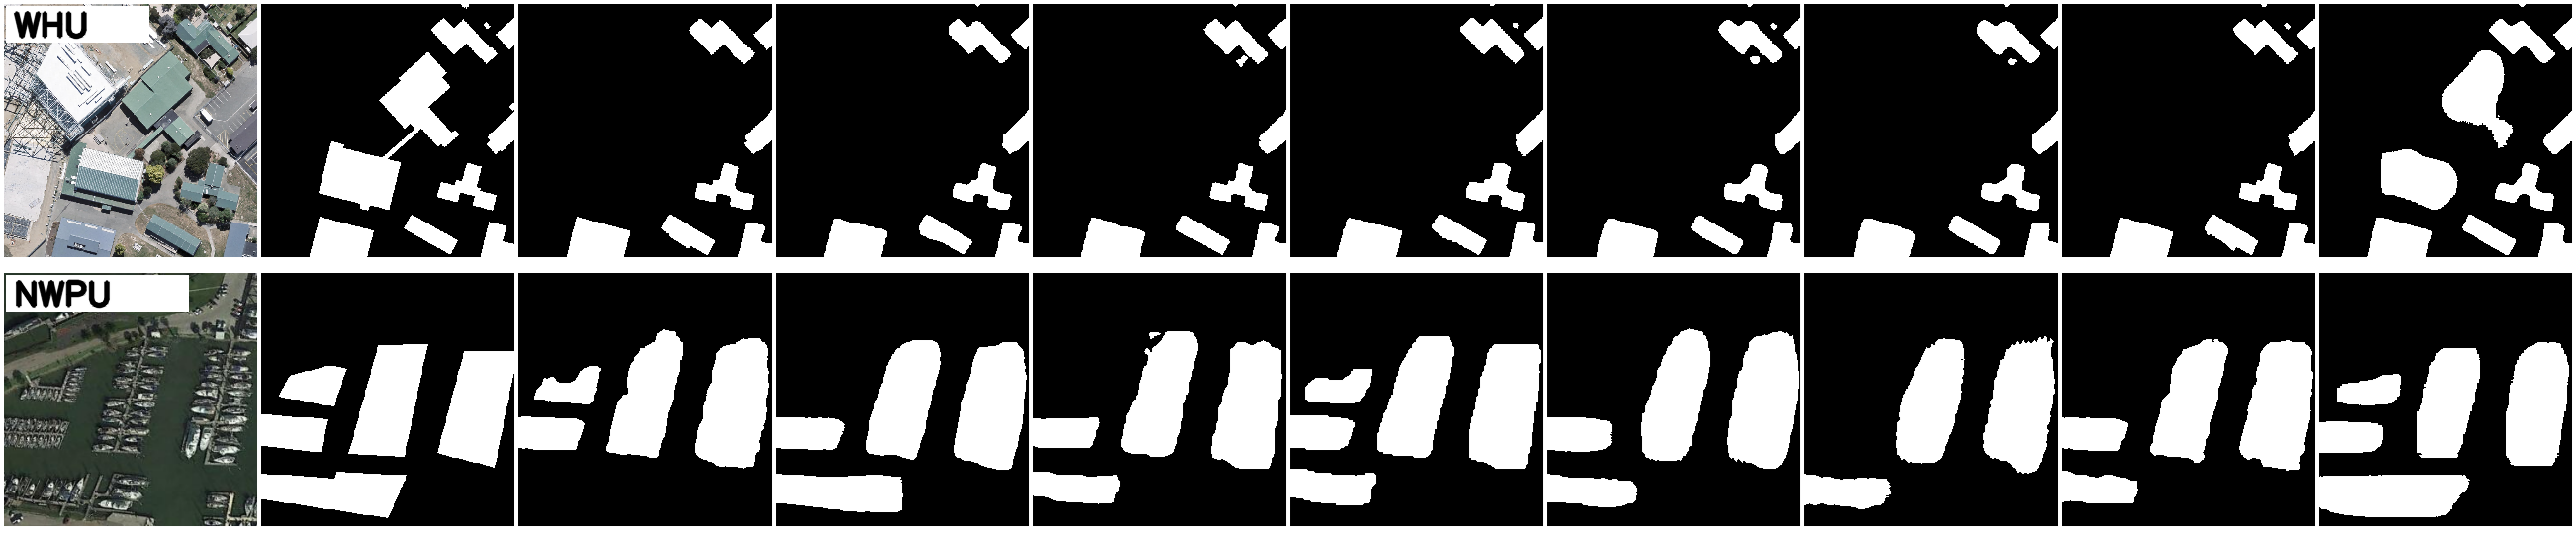
\includegraphics[width=\textwidth]{viz_grid_row_combined.png}\par
\vspace{-0.15em}
{\small
\makebox[.1\textwidth][c]{Input}%
\makebox[.1\textwidth][c]{GT}%
\makebox[.1\textwidth][c]{MaskDINO}%
\makebox[.1\textwidth][c]{RSPrompter}%
\makebox[.1\textwidth][c]{CondInst}%
\makebox[.1\textwidth][c]{YOLO11}%
\makebox[.1\textwidth][c]{HTC}%
\makebox[.1\textwidth][c]{Mask R-CNN}%
\makebox[.1\textwidth][c]{M2F}%
\makebox[.1\textwidth][c]{Ours}\par}
\vspace{-0.3em}
\caption{Qualitative comparison of existing methods and our PromptMiner-SAM2 on the WHU and NWPU VHR-10 datasets.}
\label{fig:qualitative}
\end{figure*}

\begin{table*}[!t]
\caption{Comparative analysis on the WHU and NWPU VHR-10 datasets. It reports AP / AP$_{50}$ / AP$_{75}$ for Bbox and Mask.}
\label{tab:comparison}
\centering
\small
\begingroup
\setlength{\tabcolsep}{3pt}
\renewcommand{\arraystretch}{1.08}
\begin{tabular}{llcccc}
\toprule
& & \multicolumn{2}{c}{WHU} & \multicolumn{2}{c}{NWPU VHR-10} \\
\cmidrule(lr){3-4}\cmidrule(lr){5-6}
& & Bbox (\%) & Mask (\%) & Bbox (\%) & Mask (\%) \\
\cmidrule(lr){3-3}\cmidrule(lr){4-4}\cmidrule(lr){5-5}\cmidrule(lr){6-6}
Type & Method & \metricheader & \metricheader & \metricheader & \metricheader \\
\midrule
\multirow{5}{*}{\textit{CNN}} & Mask R-CNN~\cite{maskrcnn} & \metrictriplet{70.9}{89.9}{80.9} & \metrictriplet{68.2}{90.0}{80.0} & \metrictriplet{65.4}{90.2}{78.9} & \metrictriplet{63.0}{90.1}{71.2} \\
& MS R-CNN~\cite{msrcnn} & \metrictriplet{68.8}{89.4}{80.0} & \metrictriplet{67.7}{89.6}{79.5} & \metrictriplet{67.8}{94.3}{83.8} & \metrictriplet{64.7}{93.6}{\textbf{80.8}} \\
& HTC~\cite{htc} & \metrictriplet{72.7}{90.6}{82.5} & \metrictriplet{69.2}{90.7}{81.6} & \metrictriplet{58.9}{86.9}{67.7} & \metrictriplet{51.3}{84.6}{53.3} \\
& CondInst~\cite{condinst} & \metrictriplet{74.2}{90.0}{82.4} & \metrictriplet{69.7}{90.2}{80.9} & \metrictriplet{65.0}{90.1}{79.6} & \metrictriplet{62.8}{90.7}{68.1} \\
& YOLO11s-seg~\cite{yolo11} & \metrictriplet{\textbf{76.7}}{91.2}{\textbf{85.4}} & \metrictriplet{66.8}{91.3}{79.1} & \metrictriplet{71.0}{\textbf{94.4}}{79.5} & \metrictriplet{63.9}{93.9}{67.3} \\
\midrule
\multirow{5}{*}{\textit{GSM}} & Mask2Former~\cite{mask2former} & \metrictriplet{61.4}{82.7}{70.7} & \metrictriplet{64.5}{84.1}{75.6} & \metrictriplet{60.3}{77.9}{66.8} & \metrictriplet{61.5}{84.9}{67.8} \\
& MaskDINO~\cite{maskdino} & \metrictriplet{73.3}{90.8}{82.7} & \metrictriplet{73.3}{90.3}{82.5} & \metrictriplet{65.7}{88.9}{74.2} & \metrictriplet{65.8}{89.6}{71.5} \\
& RS4D-box~\cite{rs4d} & \metrictriplet{64.5}{87.6}{74.7} & \metrictriplet{64.1}{87.8}{75.2} & \metrictriplet{57.0}{82.5}{65.4} & \metrictriplet{54.3}{80.1}{57.6} \\
& RSIISN~\cite{rsiisn} & \metrictriplet{74.1}{90.0}{84.4} & \metrictriplet{72.1}{90.1}{83.9} & \metrictriplet{66.7}{91.5}{78.4} & \metrictriplet{62.9}{89.7}{67.1} \\
& RSPrompter~\cite{rsprompter} & \metrictriplet{72.5}{91.0}{81.7} & \metrictriplet{72.5}{\textbf{92.0}}{82.9} & \metrictriplet{70.3}{93.6}{81.0} & \metrictriplet{66.1}{92.7}{70.6} \\
\midrule
Ours & PromptMiner-SAM2 & \metrictriplet{76.4}{\textbf{91.5}}{\textbf{85.4}} & \metrictriplet{\textbf{73.4}}{91.4}{\textbf{85.5}} & \metrictriplet{\textbf{73.4}}{94.0}{\textbf{84.2}} & \metrictriplet{\textbf{68.3}}{\textbf{94.5}}{74.6} \\
\bottomrule
\end{tabular}
\endgroup
\end{table*}

\begin{table}[!t]
\caption{Prompt-path and UDR module ablation on the NWPU VHR-10 dataset, where $P$, $B$, and $M$ denote point, box, and dense shape prompts, respectively, and UDR is the uncertainty-guided decoder-tail refiner.}
\label{tab:ablation}
\centering
\small
\setlength{\tabcolsep}{3pt}
\begin{tabular}{lcccccc}
\toprule
& \multicolumn{3}{c}{Bbox (\%)} & \multicolumn{3}{c}{Mask (\%)} \\
\cmidrule(lr){2-4}\cmidrule(lr){5-7}
Variant & AP & AP$_{50}$ & AP$_{75}$ & AP & AP$_{50}$ & AP$_{75}$ \\
\midrule
$P$ & 71.81 & 93.60 & 81.89 & 63.15 & 92.56 & 67.73 \\
$B$ & 72.14 & \textbf{94.34} & 82.24 & 65.25 & 94.12 & 69.02 \\
$P{+}B$ & 71.74 & 93.52 & 81.68 & 66.94 & 93.93 & 72.73 \\
$P{+}B{+}M$ & \textbf{73.76} & 93.80 & \textbf{84.69} & 66.35 & 93.66 & 71.61 \\
$P{+}B{+}M$ + UDR & 73.43 & 93.96 & 84.16 & \textbf{68.28} & \textbf{94.53} & \textbf{74.61} \\
\bottomrule
\end{tabular}
\end{table}

The model is implemented in PyTorch and trained on four NVIDIA RTX 3090 GPUs. 
Each GPU processes one image, with two gradient-accumulation steps yielding an effective batch size of eight. 
Both benchmarks are initialized from SAM2 Hiera-Base+ weights, with the Hiera backbone frozen and the adaptation modules, prompt pathway, and mask decoder trained.
Training uses AdamW with an initial learning rate of $5\times10^{-4}$ and cosine annealing. The objective joins the detection, coarse-shape, and final instance-mask losses. In particular, as shown in Table~\ref{tab:k-sensitivity}, $K=64$ is selected for all subsequent experiments because it achieves the best overall performance under a common development protocol.




\subsection{Comparative Analysis}
\looseness=-1 The proposed PromptMiner-SAM2 is compared with 10 representative
instance-segmentation methods. Table~\ref{tab:comparison} groups them into convolutional neural network (CNN) and global sequence modeling (GSM) methods. CNN covers two-stage, one-stage, and cascade designs, whereas GSM includes Transformer-based mask prediction and foundation-model adaptation methods.

It can be concluded from Table~\ref{tab:comparison} that our method obtains
the highest mask AP on both datasets, by 0.1 and 2.2 percentage points over the strongest competitors. On the WHU dataset, it also gives the best mask AP$_{75}$, while its bbox AP is 76.4\% versus 76.7\% for YOLO11s-seg. On the NWPU VHR-10 dataset, it attains the best bbox AP, bbox AP$_{75}$, mask AP, and mask AP$_{50}$. Although its mask AP$_{75}$ trails the best overall result, it exceeds every GSM method.

Figure~\ref{fig:qualitative} shows qualitative results. Compared with other methods, our method separates touching building roofs on the WHU dataset and reduces erroneous merging of adjacent instances on the NWPU VHR-10 dataset.

\subsection{Ablation Study}
\vspace{-0.35em}
Point-only $P$ serves as the baseline in Table~\ref{tab:ablation}. Adding box prompt $B$ raises mask AP/AP$_{50}$ from 63.15\%/92.56\% to 65.25\%/94.12\%. 
The box specifies the candidate extent, and the gain indicates more reliable foreground--background separation.
Combining $P{+}B$ reaches 66.94\% mask AP and 72.73\% AP$_{75}$ while bbox AP remains unchanged.
This result suggests that the two prompt types provide complementary mask-decoding constraints.
After $M$ is added, bbox AP/AP$_{75}$ rise from 71.74\%/81.68\% to 73.76\%/84.69\%, but mask AP/AP$_{75}$ are 66.35\%/71.61\%. 
This contrast indicates that the coarse shape supports region-level localization while boundary ambiguity remains. 
UDR then raises mask AP/AP$_{75}$ to 68.28\%/74.61\% with comparable bbox AP. It updates only low-confidence mask pixels using local decoder features and instance context. The higher mask scores with comparable bbox AP indicate that this targeted update improves mask delineation without materially affecting candidate localization.

\vspace{-1.5\baselineskip}
\section{CONCLUSION}
In this work, we present PromptMiner-SAM2, which mines SAM2 prompts from coarse shapes and selectively refines uncertain mask pixels. 
The results on the WHU and NWPU VHR-10 datasets show competitive and balanced detection and segmentation performance. 
In the future, it is a promising direction to explore prompts adaptive to object scale and scene context, particularly for improving cross-sensor transfer and delineating small or densely adjacent instances.

\bibliographystyle{IEEEbib}
\begingroup
\small
\interlinepenalty=10000
\bibliography{refs}
\endgroup
\end{document}
